\documentclass[answers]{exam}
\usepackage[utf8]{inputenc}

\title{Outlab 2: \LaTeX\ and gdb}
\author{Nikhil Manjrekar, Kartik Gokhale}
\date{Autumn 2021}

\usepackage{tabularx}
\usepackage{amsmath}
\usepackage{amsthm}
\usepackage[hmargin=1.35in,vmargin=1.25in]{geometry}
\usepackage{listings}
\usepackage{amssymb}
\usepackage{floatrow}
\usepackage{graphicx}
\usepackage{amsfonts}
\usepackage{xcolor}
\usepackage[linesnumbered,ruled]{algorithm2e}
\usepackage[noend]{algpseudocode}
\usepackage{hyperref}
\usepackage{listings}
\usepackage{paralist}
\usepackage{caption}
\usepackage{subcaption}

\pagestyle{headandfoot}
\runningheadrule
\runningfootrule 
\firstpagefootrule
\firstpagefooter{}{Page \thepage}{}
\firstpageheadrule
\firstpageheader{200050088, 200100083}{}{Software Systems Laboratory}
\runningfooter{}{Page \thepage}{}
\runningheader{200050088, 200100083}{}{Software Systems Laboratory}


\theoremstyle{definition}
\newtheorem{definition}{Definition}[section]
\setlength\parindent{0pt}
\setlength\parskip{0.8em}
\newcommand{\term}[0]{(u_n)_{n=0}^\infty}
\newcommand{\M}[0]{\textbf{M}}

\newcounter{list}
\lstnewenvironment{mylisting}[2]{
\lstset{
    language=#1,
    numbers=left,
    breaklines=true,
    keywordstyle=\color{blue}\bfseries,
    numberstyle=\tiny\color{gray},
    commentstyle=\color{green!30!black},
}
\refstepcounter{list}
\begin{center}
    \textbf{\large{Listing \thelist: #1}}\\
    \textbf{#2}
\end{center}
}
{
\vspace{2em}
}

\begin{document}
\maketitle
\thispagestyle{empty}
\tableofcontents
\newpage
\clearpage
\pagenumbering{arabic} 
\section{Basic Theory of Linear Recurrences}
We all know about the Fibonacci Sequence, given by the recurrence
\[f_{n+2} = f_{n+1} + f_n\]
and initialised as $f_0 = 0, f_1 = 1$. This is an instance of what is called a Linear Recurrence Sequence, or LRS.
\begin{definition}\label{defn:one}
 LRS $(u_n)_{n=0}^\infty$ of order k over field F is the sequence determined by the recurrence \begin{equation}\label{eqn:one}u_{n+k}=\sum_{j=0}^{k-1}a_ju_{n+j}\end{equation} for integers $n\geq 0$ with $a_0\ldots ,a_k \in \mathbb{F}, a_0 \neq 0$,and an initialisation vector 
 \begin{equation}
     \begin{bmatrix}u_0 \ldots u_{k-1} \end{bmatrix}^T \in \mathbb{F}^{k\times 1}
\end{equation}
\end{definition}
\noindent Thanks to Definition \ref{defn:one}, when we say that we are given $\term$ of order k over F, we actually
mean that we are given the 2k constants $a_0 \ldots a_{k-1}, u_0 \ldots u_{k-1} \in \mathbb{F}$. 

The Fibonacci sequence shows up a lot in pop culture and DSA assignments, however, the study of LRS is a vast subject in its own right, with applications in software verification, quantum computing, formal languages, statistical physics, combinatorics, and theoretical biology, to name a few.
\subsection{Computing terms of an LRS}
For a fixed k, assuming we can do arithmetic operations in $\mathbb{}$ in constant time, how long does it take to compute the $n^{th}$ term of a given LRS?

\begin{algorithm}
\caption{Naive first attempt $\mathsf{naive}$}\label{alg:one}
\KwData{LRS $\term, n$}
\KwResult{$u_n$}
\If{$n<k$}{
      \textbf{return} $u_n$
}
\textbf{return} $\Sigma_{j=0}^{k-1}a_j\cdot\mathsf{naive}(\term,n-k+j)$
\end{algorithm}

By the way, notice the use of \verb|\mathsf| to write ``$\mathsf{naive}$". This algorithm, unfortunately, is painfully
inefficient: as you can see, the number of recursive calls will be exponentially many in n. This
immediately prompts a more ``bottom-up"\footnote{Not to be confused with the drinking phrase} approach: we start from the first k terms, use them to compute the next term, and iterate this way upto $n$. This takes $\mathcal{O}(n)$ iterations.

But we can do better, in fact, we only need $\mathcal{O}$(log $n)$ iterations.\footnote{In complexity analysis, the base of the logarithm is implicitly taken as 2} 

Technically, even Algorithm \ref{alg:two} is \textit{inefficient}: when we analyse complexity, we do it with respect to the size of the \textit{bit representation} of the input, i.e. how many bits it takes to specify the input. An integer $n$ takes log $n$ bits to represent, so the parameter for describing complexity is not n, but $\eta$ = log $n$
\newpage
\begin{algorithm}
\caption{Bottom up dynamic programming approach $\mathsf{bottomup}$}\label{alg:two}
\KwData{LRS $\term, n$}
\KwResult{$u_n$}
\If{$n<k$}{
      \textbf{return} $u_n$
}
circularArray $\leftarrow$ \{$u_0,\ldots u_{k-1}$\} \\
arrayStartIndex $\leftarrow$ 0 \\
$n_{last} \leftarrow  k-1 $ \\
\While{$n_{last}<n$}{
    nextTerm $\leftarrow \Sigma_{j=0}^{k-1}a_j\cdot$ circularArray[(arrayStartIndex + j)\%k]\\
    circularArray[arrayStartIndex] $\leftarrow$ nextTerm \\
    arrayStartIndex  $\leftarrow$ (arrayStartIndex + 1)\%k \\
    $n_{last}\leftarrow n_{last}+1$
}
\textbf{return} circularArray[(arrayStartIndex + k - 1)\%k]
\end{algorithm}
Yes, we can compute the $n^{th}$ term with  $\mathcal{O}(\eta)$ operations, and the trick here is a method called
\textbf{iterated squaring}. Given an LRS $\term$, define its companion matrix $\M \in F^{k\times k}$ as
\begin{equation}\label{eqn:two}
    \M = 
    \begin{bmatrix}
    & 0 & 1 & 0 & \ldots & 0 \\
    & 0 & 0 & 1 & \ldots & 0 \\
    & \vdots & \vdots & \vdots & \ddots & 0 \\
    & 0 & 0 & 0 & \ldots & 1 \\
    & a_0 & a_1 & a_2 & \ldots & a_{k-1}
    \end{bmatrix}
\end{equation} 
Compare equations \ref{eqn:one} and \ref{eqn:two} and observe that
\begin{equation}
    \M^n = \begin{bmatrix} u_0 \\ \vdots \\ u_{k-1}\end{bmatrix}
    = \begin{bmatrix} u_n \\ \vdots \\ u_{n+k-1}\end{bmatrix}
\end{equation} 
Iterated squaring hinges on this ridiculously trivial observation: consider the (unique!) binary representation of n:  if you append a 0 to it, it becomes $2n$, if you append a 1, it becomes $2n + 1$. \\
Given \M, to compute $\M^n$, all we have to do is start with \textbf{I}, read the binary representation of $n$ from
most to least significant: if at some point we have $\M^j, \M^j \cdot\M^j = \M^{2j} , \M^{2j}\cdot\M = \M^{2j+1}$ 

In Algorithm \ref{alg:three}, we use a data structure called a stack. The constant time operations it supports are

\begin{compactitem}
    \item pushing an element onto the top of the stack
    \item popping an element from the top of the stack (i.e. deleting the topmost element)
    \item reading the topmost element
    \item checking whether the stack is empty
\end{compactitem}
As you can see, it's Last In, First Out.

The division while loop gets the bits of n from least to most significant, the iterated square while loop uses the bits from most to least significant. A stack fits the bill.
\begin{algorithm}
\caption{Iterated squaring approach $\mathsf{efficient}$}\label{alg:three}
\KwData{LRS $\term, n$}
\KwResult{$u_n$}
quotient $\leftarrow$ n \\
operationStack  $\leftarrow$ \{\} \\
\M $\leftarrow$   companion($\term$) \\
x $\leftarrow$ $\begin{bmatrix} u_0 \ldots u_{k-1} \end{bmatrix}^T$ \\
\textbf{A} $\leftarrow$ \textbf{I}$_{k\times k}$ \\
\While{quotient $\neq 0$}{
    push(operationStack, quotient\%2) \\
    quotient $\leftarrow$ quotient/2
}
\While{operationStack $\neq \{\}$}{
    \textbf{A} $\leftarrow$ \textbf{A}$\cdot$\textbf{A} \\\
    \If{top(operationStack) = 1}{
      \textbf{A} $\leftarrow$ \textbf{A}$\cdot$\textbf{M}
        }  
    pop(operationStack)
}
\textbf{y} $\leftarrow$ \textbf{Ax} \\
\textbf{return} \textbf{y}[0]

\end{algorithm}
\subsection{Problems associated with LRS}
Surprisingly, the following rather simple decision problem\footnote{Given an arbitrary input, answer a particular question about it with Yes or No}, referred to as the Skolem problem, has been open for the last eight decades or so.
\begin{definition}[Skolem Problem]
 For the arbitrary LRS $\term$ whose description is given as input, does there exist an integer $n \geq 0$ such that $u_n = 0$?
\end{definition}
This has a bunch of equivalent formulations, and by being open, we mean that nobody really knows of an algorithm that can decide it (the algorithm should terminate and give the correct answer for all possible inputs), or whether there is such an algorithm at all. 

We can also consider another related problem for LRS over fields where the $>$ operator is defined:
\begin{definition}[Positivity Problem]
  For the arbitrary LRS $\term$ whose description is given as input, is it the case that for all integers $n \geq 0$ such that $u_n \geq 0$?
\end{definition}
Deciding even special cases of these problems (i.e. restricting what kind of LRS can be fed as
input) requires sophisticated maths, like Kronecker's theorem on Diophantine approximations, [\cite{bourbaki1966elements},
Chap. 7, Sec. 1.3, Prop. 7], and profound properties of ``algebraic" numbers \cite{mignotte1982some} and then some more mathematical arsenal \cite{bell2007positivity, renegar1992computational}. \\

If you found this short write up interesting, \href{https://fmindia.cmi.ac.in/update2013/presentations/S-Akshay.pdf}{here} is a survey talk about the problem, given not so long ago.
\section{Programming}
\subsection{Output}
\verb|(gdb) print operations|\\
\verb|$1 = std::stack wrapping: std::deque with 9 elements = {0, 1, 1, 0, 1, 0, 1, 0, 1}|

\verb|(gdb) print working|\\
\verb|$2 = std::vector of length 2, capacity 2 = {std::vector of length 2, capacity 2 =|\\
\verb|{1, 0} ,std::vector of length 2, capacity 2 = {0, 1}}|
\subsection{Table}
Number chosen = 342
\begin{table}[H]
\begin{tabularx}{0.8\textwidth} { 
  | >{\raggedright\arraybackslash}X 
  | >{\centering\arraybackslash}X 
  | >{\raggedleft\arraybackslash}X | }
 \hline
 \textbf{operations} & \textbf{working} \\ 
 \hline
 \{0, 1, 1, 0, 1, 0, 1, 0, 1\} & \{1, 0, 0, 1\} \\ 
 \hline
 \{0, 1, 1, 0, 1, 0, 1, 0\} & \{0, 1, 1, 1\} \\ 
 \hline
 \{0, 1, 1, 0, 1, 0, 1\} & \{1, 1, 1, 2\} \\ 
 \hline
 \{0, 1, 1, 0, 1, 0\} & \{3, 5, 5, 8\} \\ 
 \hline
 \{0, 1, 1, 0, 1\} & \{34, 55, 55, 88\} \\ 
 \hline
 \{0, 1, 1, 0\} & \{6765, 10946, 10946, 17711\} \\ 
 \hline
 \{0, 1, 1\} & \{1.6e+8, 2.7e+8 ,2.7e+8, 4.3e+8\} \\ 
 \hline
 \{0, 1\} & \{1.6e+17, 2.6e+17, 2.6e+17, 4.2e+17\} \\ 
 \hline
 \{0\} & \{1.5e+35,
    2.4e+35,2.4e+35, 3.9e+35\} \\ 
 \hline
 \{\} & \{8.22e+70,
    1.3e+71 1.3e+71, 2.1e+71\} \\ 
 \hline
\end{tabularx}
\caption{Printing everything!}
\end{table}

\subsection{Screenshots}
\begin{figure}[H]
\centering
    \begin{floatrow}
    \ffigbox[0.50\textwidth]{\caption{Screenshot 1}}{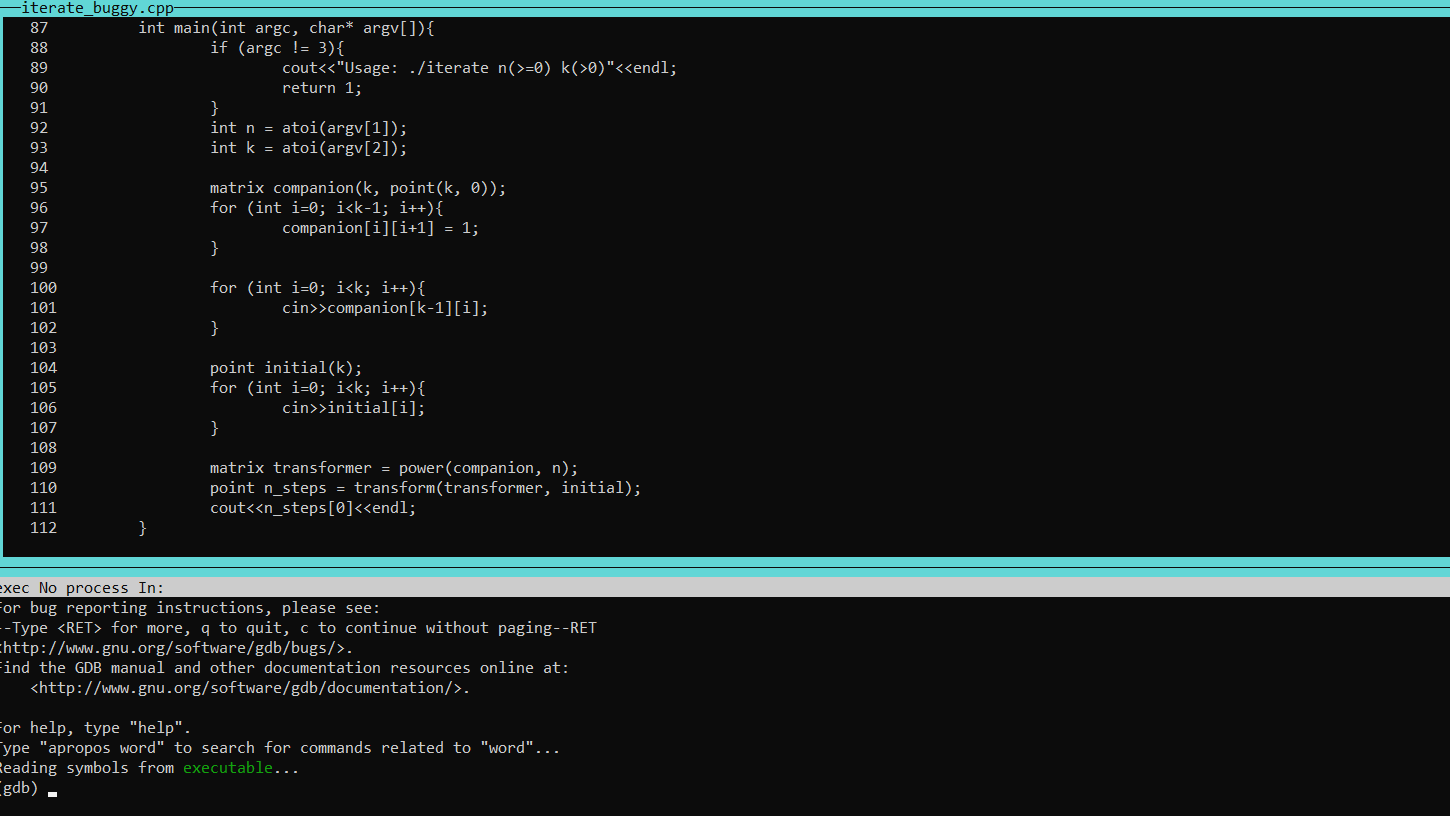
\includegraphics[width=0.50\textwidth]{1.png}}
    \ffigbox[0.50\textwidth]{\caption{Screenshot 2}}{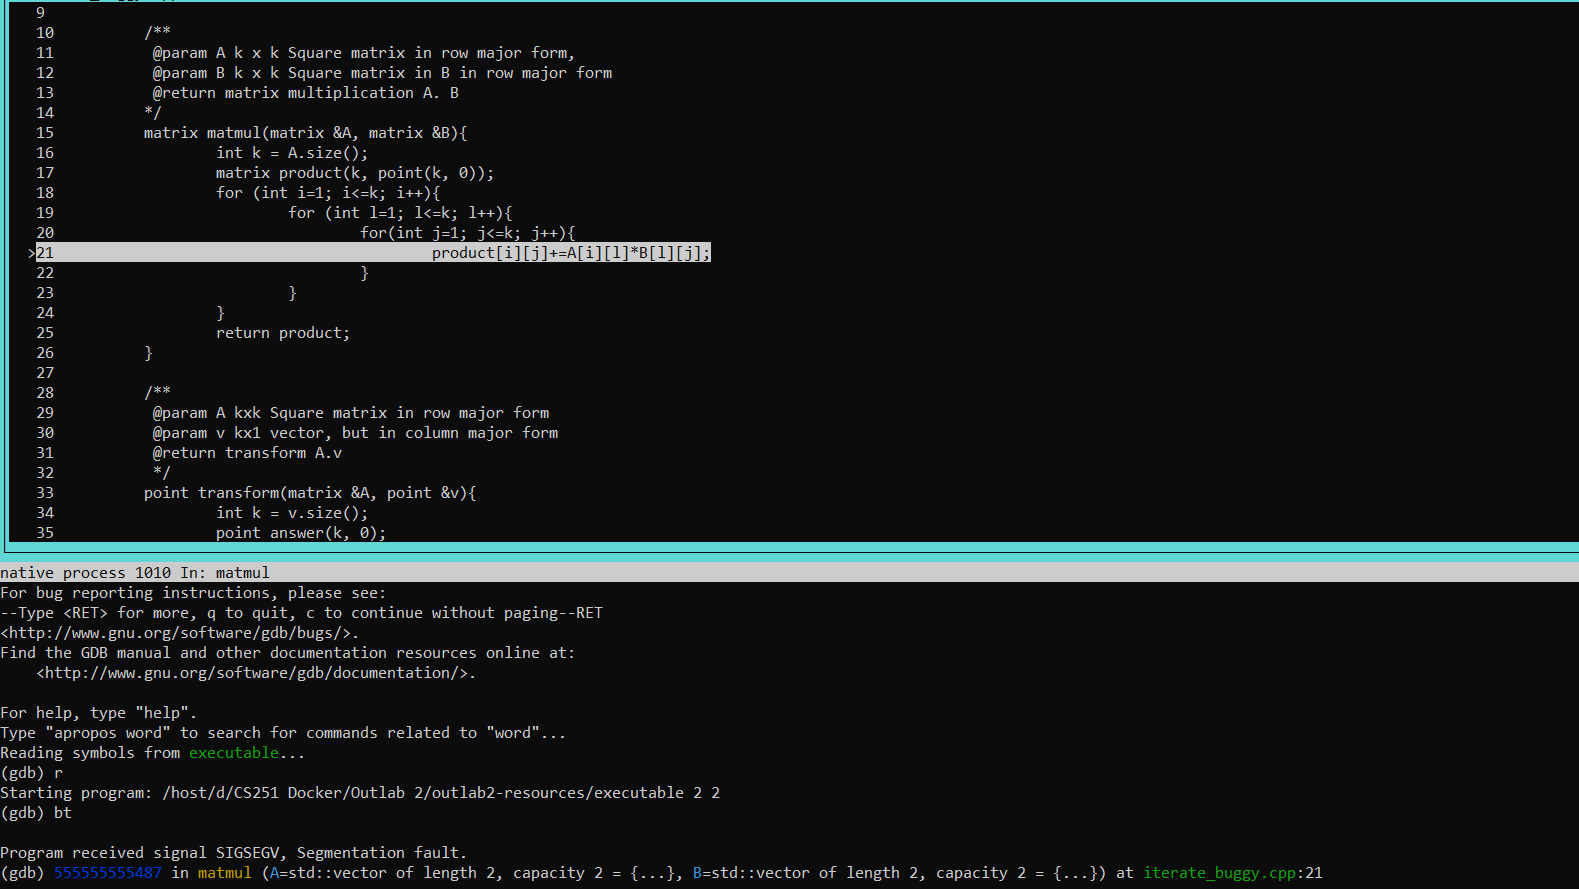
\includegraphics[width=0.50\textwidth]{2.png}}
    \end{floatrow}
\end{figure}


\newpage
\section{Hints and Tips}

\label{list:one}
\begin{mylisting}{[LaTeX]TeX }{Packages imported in the original}
\documentclass{article}
\usepackage[utf8]{inputenc}
\usepackage{hyperref}
\usepackage{fancyhdr}
\usepackage{enumitem}
\usepackage{amsmath}
\usepackage{amsthm}
\usepackage{amssymb}
\usepackage[linesnumbered, ruled, vlined]{algorithm2e}
\usepackage{listings}
\usepackage{xcolor}
\usepackage{floatrow}
\usepackage{graphics}
\bibliographystyle{plainurl}
\bibliography{biblio}
\end{mylisting}

The packages used are mentioned in Listing  \hyperref[list:one]{1}
\bibliographystyle{plainurl}
\bibliography{biblio}


\end{document}
